\documentclass[12pt]{article}

\usepackage[utf8]{inputenc}
\usepackage[margin=0.6in]{geometry}

\usepackage{amsmath}
\usepackage{graphicx}
\usepackage{booktabs}

\newcommand{\D}[2]{\frac{\mathrm{d}#1}{\mathrm{d}#2}}
\newcommand{\pfrac}[2]{\left(\frac{#1}{#2} \right)}
\newcommand{\ex}[1]{\left\langle#1\right\rangle}

\newcommand{\pdiff}[2]{\frac{\partial #1}{\partial #2}}
\newcommand{\cpdiff}[3]{\left(\pdiff{#1}{#2}\right)_{#3}}

\begin{document}

\section{Photon Walk}

\subsection{}

In any number of dimensions, if the random walk is gaussian and each scatter causes a displacement \(\ell\), we have a simple (but extremely bad) intuition for the process. The total displacement, in our toy example, is 

Let the x coordinate after \(N\) steps be the random variable \(x\), and \(dx_i\) be the change in \(x\) at the \(i^{\mathrm{th}}\) scattering. If each scatter is independent of the last (and time), \(x = \sum_1^{N} dx_i\) is a sum over iid random variables so that \(x\) tends to a gaussian as \(N\) becomes large. The \(dx_i\) have mean zero, so \(x\) has mean zero and \(\sigma_x = \sqrt{N\sigma_{dx}}\)

Applying the same treatment to \(y\) and \(z\), the distance traveled from the origin is the random variable \(r = \sqrt{x^2 + y^2 + z^2}\). Notice that \(x\), \(y\), and \(z\) are not independent because the joint probability density of \(dx_i\), \(dy_i\), and \(dz_i\) must be spherically symmetric. However, if we take for granted that \(x\), \(y\), and \(z\) are independent (or at least independent enough) we have that \(r\) is \(\chi\)-distributed, with mean proportional to \(\sigma_x\). We now have \( \left\langle r \right\rangle \propto \sqrt{N\sigma_{dx}}  \), which suggests that to travel a particular distance R, \(   \left\langle N \right\rangle \propto (R/\sigma_{dx})^2\).

All that remains is to show \(\sigma_{dx} \propto \ell\). This will depend on the specifics of how \(dx_i\) is distributed, but seems plausible. For example, a 1D discrete random walk has \(\sigma_{dx} = \sqrt{\frac{1}{2}\ell^2 + \frac{1}{2}(-\ell)^2} = \ell\)

\subsection{}

Below, we have the results of the prescribed simulation, where at each iteration, the photon jumps to a random point on the unit sphere centered at its previous location. We plot the number of iterations required for the photon to travel fifty units from the origin after \(10^5\) runs.

\begin{center}
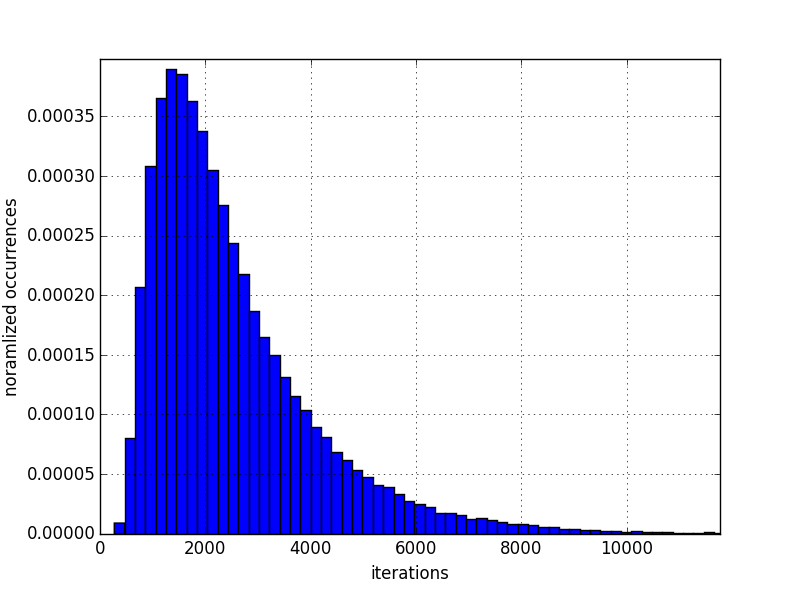
\includegraphics[scale=.7]{png/photon_walk.png}
\end{center}

The distribution has a mean of 2526.37 steps, a median of 2101 steps, and a standard deviation of 1601.14 steps. The mean is suggestively close to \(50^2\), which we expect from the previous section. One might expect that that lightcurve for an opaque body that sees a sudden injection of photons from deep inside itself would have this shape because the number of iterations required for the photon to escape, in this model, should be directly proportional to the time required for the photon to escape. 

A little more realistically, photons don't travel exactly their mean free path after every scattering event. A better model might be to draw the free path distance from an exponential distribution of mean equal to the mean free path, on the assumption that the number of scattering events in a given time is poisson.


\section{Adiabatic Gradient for Combined Ideal and Photon Gases}

\subsection{}

\begin{align*}
(1-\beta)P &= \frac{1}{3}aT^4 \\
\implies \frac{\partial}{\partial T} (P-\beta P) &= \frac{4}{3}a T^3 \\
\implies \frac{\partial P}{\partial T} - \pdiff{\beta}{T}P - \pdiff{P}{T}\beta &= \frac{4}{T}(1-\beta)P
\end{align*}

At constant \(P\), this becomes

\[ \cpdiff{\beta}{T}{P} = -\frac{4}{T}(1-\beta)
\]

\subsection{}





\end{document}